% !TeX root = mos-he.tex

%%%%%%%%%%%%%%%%%%%%%%%%%%%%%%%%%%%%%%%%%%%%%%%%%%%%%%%%%%%%%%%%

\begin{prob}{להכפיל את הדיוק}{}{(Doubling you accuracy)}
You are given two rods of lengths $L_1<L_2$ and a measuring instrument whose possible error is given by a normal distribution with mean $0$ and variance $\sigma^2$. The lengths of the two rods can be measured by measuring each one separately. Is there a more accurate method?
\end{prob}

\solution{}

\begin{figure}[bt]
\begin{center}
\begin{tikzpicture}
\draw (0,0) -- ++(6,0) -- ++(0,12pt) -- ++(-6,0) -- cycle;
\draw[<->] (0,24pt) --
  node[fill=white] {$\scriptstyle L_1+L_2$} ++(14,0);
\draw (6,0) -- ++(8,0) -- ++(0,12pt) -- ++(-8,0) -- cycle;
\begin{scope}[yshift=-48pt]
\draw (0,0) -- ++(8,0) -- ++(0,12pt) -- ++(-8,0) -- cycle;
\draw[yshift=12pt] (0,0) -- ++(0,12pt) -- ++(6,0) -- ++(0,-12pt);
\draw[<->] (6,20pt) --
  node[fill=white] {$\scriptstyle L_2-L_1$} ++(2,0);
\end{scope}
\end{tikzpicture}
\end{center}
\caption{Measuring the lengths of two rods}\label{f.rods}
\end{figure}
Place the rods end-to-end and measure $L_s=L_1+L_2$ and then place the rods side-by-side and measure $L_d=L_2-L_1$ (Figure~\ref{f.rods}). Compute $L_1,L_2$:
\begin{eqn}
\textstyle\frac{1}{2}(L_s-L_d)=\frac{1}{2}((L_1+L_2)-(L_2-L_1))&=&L_1\\
\textstyle\frac{1}{2}(L_s+L_d)=\frac{1}{2}((L_1+L_2)+(L_2-L_1))&=&L_2\,.
\end{eqn}
The errors in the measurements are $e_s, e_d$ so the errors in the results are:
\begin{eqn}
\textstyle\frac{1}{2}((L_s+e_s)-(L_d+e_d))&=&L_1+\textstyle\frac{1}{2}(e_s-e_d)\\
\textstyle\frac{1}{2}((L_s+e_s)+(L_d+e_d))&=&L_2+\textstyle\frac{1}{2}(e_s+e_d)\,.
\end{eqn}
Since the mean of the measurement instrument is $0$, the mean of the errors of these measurements is also zero. The variance is reduced to half its previous value:\footnote{We use the fact that the measurements are independent so the covariance is zero.}
\begin{eqn}
\mathrm{Var}\left(\textstyle\frac{1}{2}\left(e_s-e_d\right)\right)&=&
  \textstyle\frac{1}{4}(\sigma^2+(-1)^2\sigma^2)=\frac{1}{2}\sigma^2\\
\mathrm{Var}\left(\textstyle\frac{1}{2}(e_s+e_d)\right)&=&
  \textstyle\frac{1}{4}( \sigma^2+\sigma^2)=\frac{1}{2}\sigma^2\,.
\end{eqn}


%%%%%%%%%%%%%%%%%%%%%%%%%%%%%%%%%%%%%%%%%%%%%%%%%%%%%%%%%%%%%%%%

\begin{prob}{משוואות ריבועיות אקראיות}{S}{(Random quadratic equations)}

Consider the quadratic equation $x^2+2bx+c=0$ defined on $[-B,B]\times[-B,B]$ for $B\geq 1$.

\que{1} What is the probability that the roots are real?

\que{2} As $B\rightarrow \infty$ what is the probability that the roots are real?
\end{prob}

\solution{}

\ans{1}
The roots will be real if the discriminant is non-negative $4b^2-4c\geq 0$. Figure~\ref{f.real-roots} shows a plot of the parabola $c=b^2$ where the complex roots are within the shaded area. For example, for $(b,c)=(1,2)$, $x^2+2x+2$ has complex roots (red dot) while for $(b,c)=(2,2)$, $x^2+4x+2$ has real roots (blue dot).

\begin{figure}[tb]
\begin{center}
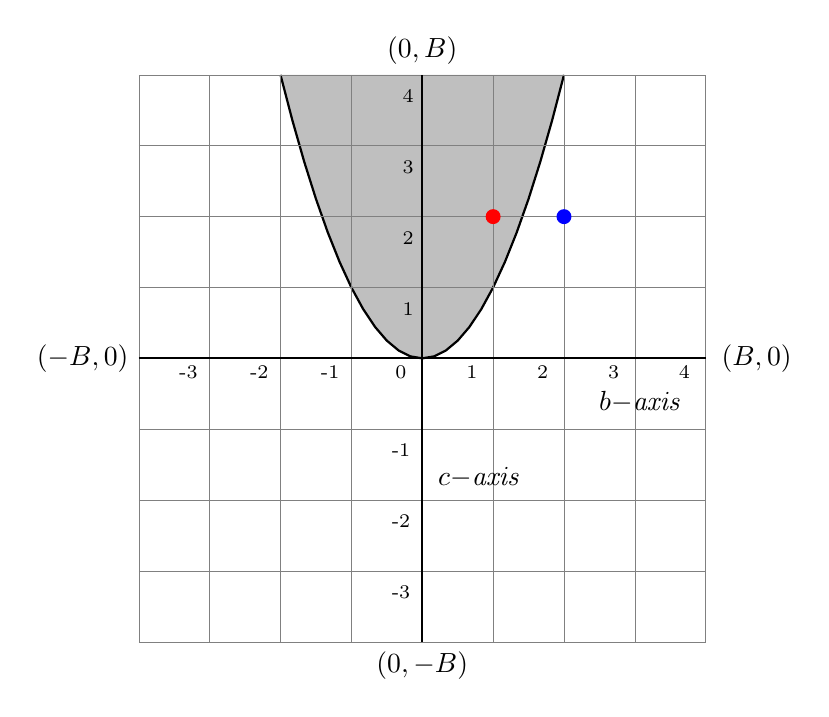
\begin{tikzpicture}[scale=.9]
\fill [white!50!gray, domain=-2:2]
      (-2, 4) -- plot ({\x}, {\x*\x}) -- (2, 4) -- cycle;
\draw [thick, domain=-2:2]
      (-2, 4) -- plot ({\x}, {\x*\x}) -- (2, 4);
\draw[help lines] (-4,-4) grid (4,4);
\draw[thick] (-4,0) -- (4,0);
\draw[thick] (0,-4) -- (0,4);
\foreach \x in {-3,...,4}
  \node at (\x-.3,-.2) {\scriptsize \x};
\foreach \y in {1,...,4}
  \node at (-.2,\y-.3) {\scriptsize \y};
\foreach \y in {-3,...,-1}
  \node at (-.3,\y-.3) {\scriptsize \y};
\draw[thick] (0,-4) node[below] {$(0,-B)$} -- 
  node[right,near start,xshift=2pt,yshift=8pt]
  {$c\mathit{-axis}$} (0,4) node[above] {$(0,B)$};
\draw[thick] (-4,0) node[left] {$(-B,0)$} --
  node[below,very near end,xshift=2pt,yshift=-8pt] 
  {$b\mathit{-axis}$} (4,0) node[right,xshift=2pt] {$(B,0)$};
\fill[red] (1,2) circle(3pt);
\fill[blue] (2,2) circle(3pt);
\end{tikzpicture}
\end{center}
\caption{For $(b,c)$ in the shaded area the roots of $c=b^2$ are complex}\label{f.real-roots}
\end{figure}

The shaded area can be computed by integration:
\[
\int_{-\sqrt{B}}^{\sqrt{B}} (B-b^2)\,db=
\left. Bb-\disfrac{b^3}{3}\right|_{-\sqrt{B}}^{\sqrt{B}}=
\left(B^{3/2}-\frac{B^{3/2}}{3}\right)-
\left(-B^{3/2}+\frac{B^{3/2}}{3}\right)=
\disfrac{4}{3}B^{3/2}\,.
\]
The total area of the range $[-B,B]\times[-B,B]$ is $4B^2$ so:
\begin{eqn}
P(\textrm{complex roots})&=&\disfrac{\frac{4}{3}B^{3/2}}{4B^2}=\disfrac{1}{3\sqrt{B}}\\
P(\textrm{real roots})&=&1-\disfrac{1}{3\sqrt{B}}\,.
\end{eqn}
\ans{2}
\[
\lim_{B\rightarrow\infty}
P(\textrm{real roots})=
\lim_{B\rightarrow\infty} \left(1-\disfrac{1}{3\sqrt{B}}\right)=
1\,.
\]

\textbf{Simulation}
\begin{verbatim}
For B =  4:
Probability of real roots = 0.8333
Proportion real roots     = 0.8271
For B = 16:
Probability of real roots = 0.9167
Proportion real roots     = 0.9205
For B = 64:
Probability of real roots = 0.9583
Proportion real roots     = 0.9582
\end{verbatim}

%%%%%%%%%%%%%%%%%%%%%%%%%%%%%%%%%%%%%%%%%%%%%%%%%%%%%%%%%%%%%%%%

\begin{prob}{הילוך מקרי דו-ממדי}{S}{(Two-dimensional random walk)}
A particle is placed at the origin of a two-dimensional coordinate system. The particle moves left or right on the $x$-axis with probabilities $1/2$ \emph{and} up or down the $y$-axis with probabilities $1/2$. Figure~\ref{f.2d-random-walk} shows a random walk of $22$ steps starting at and returning to the origin.

\que{1} What is the probability of returning to the origin in $2$ moves?

\que{2} What is the probability that the particle returns (one or more times) to the origin?

\que{3} Use Stirling's approximation to obtain an estimate of the probability for large $n$.

\begin{figure}[t]
\begin{center}
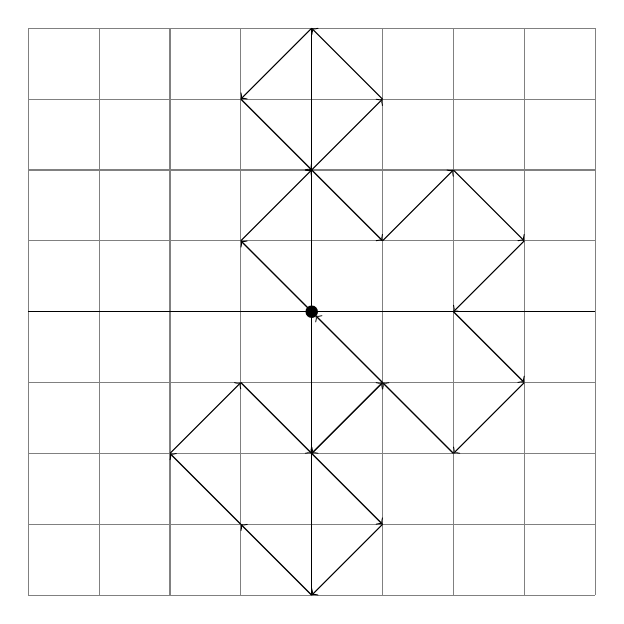
\begin{tikzpicture}[scale=.9]
\draw[color=gray] (-4,-4) grid (4,4);
\draw (-4,0) -- (4,0);
\draw (0,-4) -- (0,4);
\fill (0,0) circle[radius=2.5pt];
\draw[->] (0,0)  -- (-1,1);
\draw[->] (-1,1) -- (0,2);
\draw[->] (0,2)  -- (1,3);
\draw[->] (1,3)  -- (0,4);
\draw[->] (0,4)  -- (-1,3);
\draw[->] (-1,3) -- (0,2);
\draw[->] (0,2)  -- (1,1);
\draw[->] (1,1)  -- (2,2);
\draw[->] (2,2)  -- (3,1);
\draw[->] (3,1)  -- (2,0);
\draw[->] (2,0)  -- (3,-1);
\draw[->] (3,-1) -- (2,-2);
\draw[->] (2,-2) -- (1,-1);
\draw[->] (1,-1) -- (0,-2);
\draw[->] (0,-2) -- (1,-3);
\draw[->] (1,-3) -- (0,-4);
\draw[->] (0,-4) -- (-1,-3);
\draw[->] (-1,-3)-- (-2,-2);
\draw[->] (-2,-2)-- (-1,-1);
\draw[->] (-1,-1)-- (0,-2);
\draw[->] (0,-2) -- (1,-1);
\draw[->] (1,-1) -- (.055,-.055);
\end{tikzpicture}
\end{center}
\caption{Two-dimensional random walk}\label{f.2d-random-walk}
\end{figure}

\end{prob}

\solution{}

\ans{1}
The dots in Figure~\ref{f.two-moves} show the possible positions of the particle after two moves:
\begin{itemize}
\item The green path shows how to move to $(\pm 2, \pm 2)$ by taking two moves in the same direction. The probability is $\left(\frac{1}{4}\right)^2= \frac{1}{16}$.
\item The red path shows how to move to $(\pm 2,0)$ or $(0,\pm 2$). There are two possible paths for each one so the probability is $2\cdot\left(\frac{1}{4}\right)^2= \frac{2}{16}$.
\item The blue path shows how to move to $(\pm 1,\pm 1)$ and back to the origin. The probability is $1/16$. Since there are four paths that return to the origin the probability is $\frac{4}{16}$.
\end{itemize}
The blue paths are the only ones that return to the origin so:
\[
P(\textrm{return to origin in two moves})=\frac{4}{16}\,.
\]

\begin{figure}[tb]
\begin{center}
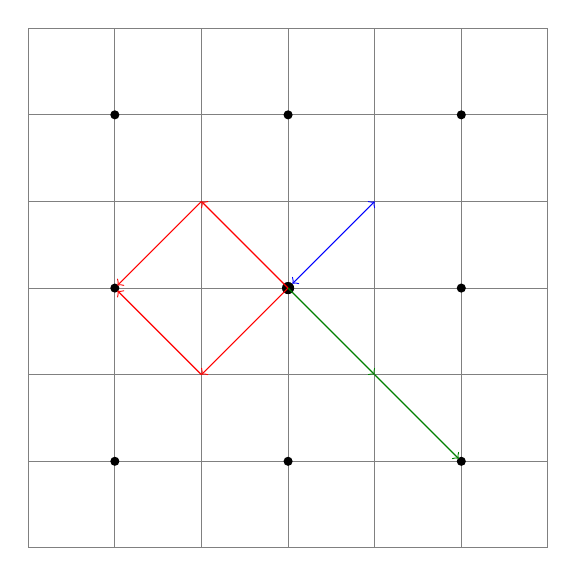
\begin{tikzpicture}[scale=1.1]
\draw[color=gray] (-3,-3) grid (3,3);
\fill (0,0) circle[radius=2pt];
\foreach \x/\y in {2/2, 2/-2, -2/2, -2/-2, 
                   0/2, 0/-2, 2/0, -2/0}
  \fill (\x,\y) circle[radius=1.5pt];
\draw[->,red] (0,0) -- (-1,-1);
\draw[->,red] (-1,-1) -- (-1.97,-.03);
\draw[<-,red] (-1.97,0.03) -- (-1,1);
\draw[<-,red] (-1,1) -- (0,0);
\draw[->,green!50!black] (0,0) -- (1,-1);
\draw[->,green!50!black] (1,-1) -- (1.97,-1.97);
\draw[<->,blue] (.05,.05) -- +(.95,.95);
%\draw[->,blue] (-0.1,0) -- +(1,1);
%\draw[->,blue] (1.1,1) -- +(-1,-1);
\end{tikzpicture}
\end{center}
\caption{Two moves of the random walk}\label{f.two-moves}
\end{figure}

\ans{3} The choices of direction for $x$ and $y$ are independent so for $2n$ moves:
\begin{equation}\label{eq.2d-1}
P_{2n}(\textrm{return to origin}) =
P_{2n}(\textrm{return to}\;x=0)\,P_{2n}(\textrm{return to}\;y=0)\,.
\end{equation}
The particle will return to the origin if and only if for both axes the number of $+1$ moves equals the number of $-1$ moves. There are ${2n \choose n}$ ways to arrange $+1$s and $-1$s so:
{
\addtolength{\arraycolsep}{-3pt}
\begin{eqnarray}
P_{2n}(\textrm{return to}\;x=0) =P_{2n}(\textrm{return to}\;y=0)&=&
\dischoose{2n}{n}\left(\disfrac{1}{2}\right)^n\left(\disfrac{1}{2}\right)^{n}\\
P_{2n}(\textrm{return to origin}) &=&
\left[\dischoose{2n}{n}\left(\disfrac{1}{2}\right)^{2n}\right]^2\\
P(\textrm{return to origin}) =
\sum_{n=1}^{\infty}P_{2n}(\textrm{return to origin}) &=&
\sum_{n=1}^{\infty}\left[\dischoose{2n}{n}\left(\disfrac{1}{2}\right)^{2n}\right]^2\,.\label{eq.2d-2}
\end{eqnarray}
}
\ans{3}
By Stirling's approximation $n! \approx \sqrt{2\pi n}\left(n/e\right)^n$:
\begin{eqn}
P_{2n}(\textrm{return to origin}) &=&
\left[\dischoose{2n}{n}
\left(\disfrac{1}{2}\right)^{2n}\right]^2 \\
&=&
\left[\disfrac{(2n)!}{(n!)^2}
\left(\disfrac{1}{2}\right)^{2n}\right]^2 \\
&\approx&
\left(\disfrac{1}{2}\right)^{4n}
\disfrac{(\sqrt{2\pi \cdot 2n})^2
         \left(2n/e\right)^{4n}}
        {(\sqrt{2\pi n})^{4}
         \left(n/e\right)^{4n}} \\
&=&\left(\disfrac{1}{2}\right)^{4n}\disfrac{4\pi n}{4\pi^2 n^2}\cdot
\disfrac{\left(n/e\right)^{4n}\cdot 2^{4n}}{\left(n/e\right)^{4n}}\\
&=& \disfrac{1}{\pi n}\\
P(\textrm{return to origin}) &=& \disfrac{1}{\pi}\sum_{n=1}^{\infty}\disfrac{1}{n}\,,
\end{eqn}
which is the \emph{harmonic series} that diverges. This means that with probability $1$ the particle returns to the origin.

\textbf{Simulation}
The simulation was run one million times instead of ten thousand times but still there is no certainty of returning to the origin:
\begin{verbatim}
Proportion returned to origin      = 0.8700
\end{verbatim}

%%%%%%%%%%%%%%%%%%%%%%%%%%%%%%%%%%%%%%%%%%%%%%%%%%%%%%%%%%%%%%%%

\begin{prob}{הילוך מקרי תלת-ממדי}{D,S}{(Three-dimensional random walk)}
A particle is placed at the origin of a three-dimensional coordinate system. The particle moves left or right on the $x$-axis with probabilities $1/2$ \emph{and} up or down the $y$-axis with probabilities $1/2$ \emph{and} in or out on the $z$-axis with probabilities $1/2$.

\que{1} What is the expectation of the number of times that the particle returns to the origin?

\textbf{Hint:} Compute the probability and then use an indicator variable.

\que{2} What is the probability that the particle will return to the origin (at least once)?

\textbf{Hint:} Use the technique from Problem~4.
\end{prob}

\solution{}

$P_{2n}$, probability of returning to the origin after $2n$ steps, is given by the analogue of Equation~\ref{eq.2d-1}:
\[
P_{2n} =
P_{2n}(\textrm{return to}\;x=0)\,P_{2n}(\textrm{return to}\;y=0\, P_{2n}(\textrm{return to}\;z=0)\,.
\]
$P_r$, the probability of returning to the origin one or more times, is given by the analogue of Equation~\ref{eq.2d-2}:
\[
P_r =\sum_{n=1}^{\infty}P_{2n} =
\sum_{n=1}^{\infty}\left[\dischoose{2n}{n}\left(\disfrac{1}{2}\right)^{2n}\right]^3\,.
\]

From Stirling's approximation:\footnote{Mosteller used $18$ terms in his computation and obtained $0.315$. My program used $500$ terms to obtain $0.3772$.}
\begin{eqn}
P_{2n} &=&
\left[\disfrac{(2n)!}{(n!)^2}
\left(\disfrac{1}{2}\right)^{2n}\right]^3 \\
&\approx&
\left(\disfrac{1}{2}\right)^{6n}
\disfrac{(\sqrt{2\pi \cdot 2n})^3
         \left(2n/e\right)^{6n}}
        {(\sqrt{2\pi n})^{6}
         \left(n/e\right)^{6n}} \\
&=&\disfrac{(4\pi n)^{3/2}}{(2\pi n)^3}=
 \disfrac{1}{(\pi n)^{3/2}}\\
P_r &=& \sum_{n=1}^{\infty}\disfrac{1}{(\pi n)^{3/2}}\approx 0.3772\,.
\end{eqn}
Let $I_k$ be the indicator variable for a return to the origin on step $k$:
\begin{equation}
I_k=
\left\{
\begin{array}{ll}
1,\quad\textrm{if particle returns to origin on step}\;k\\
0, \quad\textrm{if particle does not returns to origin on step}\;k\,.
\end{array}
\right.
\end{equation}
Then:
\[
E(\textrm{number of returns to the origin})=\sum_{n=1}^{\infty}P_{2n}\, I_{2n} = P_r\approx 0.3772\,,
\]
so the expectation of the number of returns is equal to the probability.

\que{2} Let $P_1$ be the probability that the particle returns to the origin \emph{at least once}.  From Problem~4 we know that the expectation of the number of trials until the first one where the particle \emph{does not} return to the origin is $1/(1-P_1)$. Therefore, the expectation of the number of trials for which the particle does return to the origin is one less, because the particle can return to the origin many times until finally it does not.\footnote{Mosteller's presentation is not easy to follow. I would like to thank Aaron Montgomery for clarification \L{\cite{montgomery}}.}

Let $E_r=E(\textrm{number of returns to the origin})$, then:
\begin{eqn}
E_r &=& \disfrac{1}{1-P_1} - 1\\
P_1&=& \disfrac{E_r}{1+E_r}\,.
\end{eqn}
In \ans{1} we computed that $E_r\approx 0.3772$ so:
Then:
\[
P_1 \approx 1- \disfrac{1}{1+0.3772}
\approx 0.2739\,.
\]

\textbf{Simulation}
\begin{verbatim}
Expectation of reaching origin = 0.3772
Average times reached origin   = 0.3630
Probability of reaching origin = 0.2739
Proportion reached origin      = 0.2790
\end{verbatim}

%%%%%%%%%%%%%%%%%%%%%%%%%%%%%%%%%%%%%%%%%%%%%%%%%%%%%%%%%%%%%%%%

\begin{prob}{המחט של \L{Buffon}}{D,S}{(Buffon's needle)}
Consider a needle of length $a\leq 1$ and a surface ruled with parallel lines $1$ apart. Throw the needle onto the surface. What is the probability that the needle crosses a line?\footnote{The problem has been simplified by specifying the distance between the parallel lines as $1$. We ignore the possibility that the needle lies completely along the line or just touches two lines since the probability of these events is zero.}

\textbf{Hint:} There are two independent random variables (Figure~\ref{f.buffon1}): $x$, the position of the center of the needle relative to the closest line which is uniformly distributed in the range $[0,1]$, and $\theta$, the angle formed by the needle relative to the parallel lines which is uniformly distributed in the range $[0,\pi/2]$.

\begin{figure}[tb]
\begin{center}
\begin{tikzpicture}[scale=.9]
\draw (0,0) -- (10,0);
\draw (0,4) -- (10,4);
\draw[<->] (1,0) -- node[fill=white] {$1$} (1,4);
\coordinate (center) at ($(4,-.5)+(60:1.5)$);
\node[above right,xshift=4pt] at (center) {$\theta$};
\node[above left] at (center) {$C$};
\draw[thick] (4,-.5) -- node[right,very near end] {$a$} +(60:4);
\draw[thick,dashed] ($(center)+(-2,0)$) -- +(6,0);
\draw[<->] (5.3,0) -- node[fill=white] {$x$}
  (center -| 5.3,0);
\end{tikzpicture}
\end{center}
\caption{Buffon's needle}\label{f.buffon1}
\end{figure}

\end{prob}

\solution{1}

Let $p(a)$ be the probability that a needle of length $a$ crosses a line and define the indicator variable:
\[
I_{\textrm{crosses}}=
\left\{
\begin{array}{ll}
1,\quad \textrm{if needle of length}\;a\;\textrm{crosses a line}\\
0, \quad \textrm{if needle of length}\;a\;\textrm{does not cross a line}\,.
\end{array}
\right.
\]
Then:
\begin{equation}\label{eq.buffon-probability}
E(I_{\textrm{crosses}})=1\cdot p(a) + 0\cdot (1-p(a))=p(a)\,,
\end{equation}
and the probability can be computed by computing the expectation.

Let $m$ be a line perpendicular to the parallel lines that passes through the center of the needle and let $\theta$ be the angle between the needle and a parallel line. Project the needle onto $m$ to give the line segment $\overline{CD}$. The probability that the needle will cross a line is:
\begin{equation}\label{eq.cross}
P(\textrm{needle of length}\;a,\;\textrm{angle}\;\theta\;\textrm{crosses line})=\disfrac{\overline{CD}/2}{1/2}=\disfrac{(a/2)\sin \theta}{1/2}=a\sin\theta\,.
\end{equation}

\begin{figure}[bt]
\begin{center}
\begin{tikzpicture}[scale=1.5]
\draw (0,0) coordinate (O) -- (6,0);
\draw (0,2.5) -- (6,2.5);
\draw[<->] (.7,0) -- node[fill=white,near end] {$1$} +(0,2.5);
\draw[<->] (5,0) -- node[fill=white] {$1/2$} +(0,1.25);
\coordinate (end1) at (2,-.5);
\coordinate (end2) at ($(end1)+(60:3)$);
\coordinate (center) at ($(end1)+(60:1.5)$);
\draw[thick,dotted] (O |- center) -- +(6,0);
\draw[thick,dashed] (0,1.25) -- +(6,0);
\node[right,xshift=4pt,yshift=8pt]
  at (center) {$\theta$};
%\node[left,xshift=-4pt,yshift=-8pt]
%  at (center) {$\theta$};
\draw[thick,dashed] ($(center)+(0,-2)$) --
  node[right,very near end,xshift=-2pt,yshift=15pt]
  {$m$} +(0,4.2);
\node[right] at (end1 -| center) {$D$};
\node[left] at (end2-| center) {$C$};
\draw[thick] (end1) -- 
  node[left,near end] {$a/2$} (center) --
%  node[right] {$a/2$} 
  (end2);
\draw[thick] (end1) node[above right,xshift=4pt] {$\theta$} --
  (end1 -| center) --
  node[right,yshift=4pt] {$(a\sin\theta)/2$} (center);
\draw[thick] (end2) -- (end2 -| center) -- (center);
%\draw[thick] (end2) node[below left,xshift=-4pt] {$\theta$} --
%  (end2 -| center) -- 
%  node[left] {$(a\sin \theta)/2$} (center);
\end{tikzpicture}
\end{center}
\caption{Right triangle for solving Buffon's needle problem}\label{f.buffon2}
\end{figure}

The expectation of the number of lines crossed is given by integrating over possible angles:
\begin{equation}\label{eq.buffon-integral}
E(\textrm{lines crossed}) =
  \disfrac{1}{(\pi/2)-0} \int_0^{\pi/2} a\sin \theta\,
  d\theta=\left.\disfrac{2}{\pi}\cdot a (-\cos \theta)
  \right|_0^{\pi/2}=\disfrac{2a}{\pi}\,.
\end{equation}

\solution{2} This solution is taken from \cite[Chapter~26]{proofs}.

\begin{figure}[tb]
\begin{center}
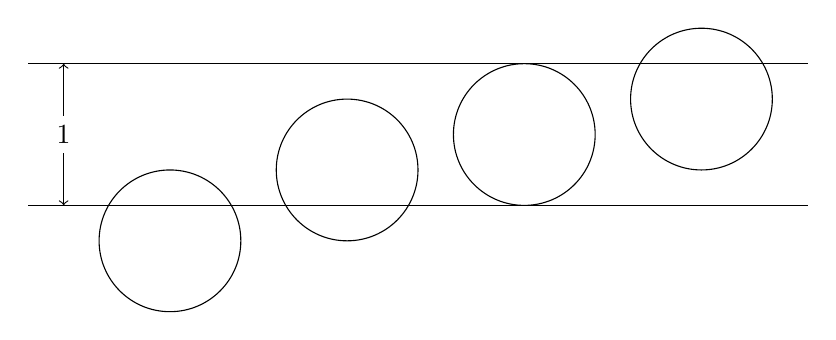
\begin{tikzpicture}[scale=.9]
\draw (0,0) -- (11,0);
\draw (0,2) -- (11,2);
\draw[<->] (.5,0) -- node[fill=white] {$1$} (.5,2);
\foreach \x/\y in {2/-.5, 4.5/.5, 7/1, 9.5/1.5}
  \draw (\x,\y) circle[radius=1];
\end{tikzpicture}
\end{center}
\caption{Solving Buffon's needle with circles}\label{f.buffon3}
\end{figure}

Let $E(x)$ be the expectation of the number of parallel lines crossed by a line $x$. Consider a line formed into a circle $C$ of \emph{diameter} $1$ and circumference $\pi$. If the circle is thrown onto the surface it will have \emph{exactly} two intersections with the lines (Figure~\ref{f.buffon3}), that is:
\begin{equation}\label{eq.buffon-2}
E(C)=2\,.
\end{equation}
Inscribe a regular polygon $Q_n$ (red) within $c$ (green) and circumscribe a regular polygon $R_n$ (blue) around $c$ (Figure~\ref{f.buffon4}). Any line (red) that $Q_n$ crosses must also cross the circle and any line (blue) that crosses the circle must also cross $R_n$. Therefore:
\begin{equation}\label{eq.buffon3}
E(Q_n)\leq E(C)\leq E(R_n)\,.
\end{equation}
Let $a_Q, a_R$ be the sums of the lengths of the sides of $Q_n,R_n$, respectively. By the linearity of expectation:
{
\addtolength{\arraycolsep}{-3pt}
\begin{eqnarray}\label{eq.buffon1a}
E(Q_n)&=&\sum_{i=1}^n E(\textrm{segments of}\;a_Q)=a_QE(1)\\
\label{eq.buffon1b}E(R_n)&=&\sum_{i=1}^n E(\textrm{segments of}\;a_R)=a_RE(1)\,. 
\end{eqnarray}
}
As $n\rightarrow\infty$ both polygons approximate the circle so:
\begin{equation}\label{eq.buffon-pi}
\lim_{n\rightarrow\infty}a_Q = \lim_{n\rightarrow\infty} a_R=\pi\,,
\end{equation}
the circumference of the circle. From Equations~\ref{eq.buffon-2}--\ref{eq.buffon-pi} we have:
\[
\renewcommand*{\arraystretch}{1.5}
\begin{array}{l}
\lim_{n\rightarrow\infty}E(Q_n)=E(C) =\lim_{n\rightarrow\infty}E(R_n)\\
E(C)=aE(1) =\pi E(1) = 2\\
E(1)=\disfrac{2}{\pi}\\
E(a)=aE(1)=\disfrac{2a}{\pi}\,.
\end{array}
\]
\begin{figure}[bt]
\begin{center}
\begin{tikzpicture}
\draw[thick,green!80!black] (0,0) circle[radius=2];
\node[draw,red,thick] (in)
  [minimum size=4cm,regular polygon,regular polygon sides=6]
  at (0,0) {};
\node[draw,blue,rotate=30,thick] (out)
  [minimum size=4.62cm,regular polygon,regular polygon sides=6]
  at (0,0) {};
\node[above left,xshift=5pt] at (in.corner 5) {$Q_n$};
\node[below right,yshift=6pt] at (out.corner 5) {$R_n$};
\draw[thick,red] (-3,-.6) -- +(6,0);
\draw[thick,blue] (-3,1.9) -- +(6,0);
\end{tikzpicture}
\end{center}
\caption{Polygons approximate a circle}\label{f.buffon4}
\end{figure}

\textbf{Simulation}

Since $\pi=2a/E$ the simulation (or actually throwing needles on a table!) can be used to obtain an approximation of $\pi$.

\begin{verbatim}
For length = 0.2:
Expectation of crossings = 0.1273
Average crossings        = 0.1308
Empirical value for pi   = 3.0581

For length = 0.5:
Expectation of crossings = 0.3183
Average crossings        = 0.3227
Empirical value for pi   = 3.0989

For length = 1.0:
Expectation of crossings = 0.6366
Average crossings        = 0.6333
Empirical value for pi   = 3.1581
\end{verbatim}

%%%%%%%%%%%%%%%%%%%%%%%%%%%%%%%%%%%%%%%%%%%%%%%%%%%%%%%%%%%%%%%%

\begin{prob}{המחט של \L{Buffon} עם רשת אופקי ואנכי}{}{\\(Buffon's needle with horizontal and vertical rulings)}

Solve Buffon's needle problem for a surface that is covered by a grid with squares of size $1\times 1$. A needle can cross a vertical line (green), a horizontal line (blue), both (red) or neither (orange) (Figure~\ref{f.buffon5}).

\begin{figure}[b]
\begin{center}
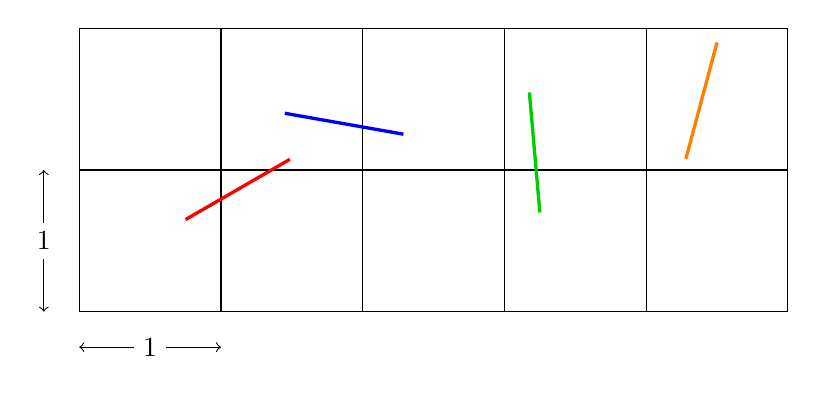
\begin{tikzpicture}[scale=.9]
\draw[step=2cm] (0,0) grid (10,4);
\draw[<->] (-.5,0) -- node[fill=white] {$1$} (-.5,2);
\draw[<->] (0,-.5) -- node[fill=white] {$1$} (2,-.5);
\foreach \x/\y/\a/\c in {
  1.5/1.3/30/red,
  2.9/2.8/-10/blue,
  6.5/1.4/95/green!80!black,
  9/3.8/-105/orange}
    \draw[color=\c,very thick] (\x,\y) -- +(\a:1.7);
\end{tikzpicture}
\end{center}
\caption{Buffon's needle with horizonal and vertical crossings}\label{f.buffon5}
\end{figure}
\end{prob}

\textbf{Hint:} Are the numbers of crossings of the horizontal and vertical lines independent?

\solution{}

The numbers of crossings of the horizontal and vertical lines are independent and expectation is linear so:
\begin{eqn}
E(\textrm{lines crossed by\ } a)&=&E(\textrm{vertical lines crossed by\ } a +
     \textrm{horizontal lines crossed by\ } a)\\
&=&E(\textrm{vertical lines crossed by\ } a) +
   E(\textrm{horizontal lines crossed by\ } a)\\
&=&\disfrac{2a}{\pi}+\disfrac{2a}{\pi}=\disfrac{4a}{\pi}\,.
\end{eqn}


%%%%%%%%%%%%%%%%%%%%%%%%%%%%%%%%%%%%%%%%%%%%%%%%%%%%%%%%%%%%%%%%

\begin{prob}{מחטים ארוכים}{D,S}{(Long needles)}

Let the length of the needle in Buffon's problem be $a>1$.

\que{1} What is the expectation of the \emph{number of crossings}?

\que{2} What is the probability that there is \emph{at least one crossing}?

\textbf{Hint:} For what angles $\theta$ is the probability a crossing $1$?

\end{prob}

\solution{}

\ans{1} Break the needle into pieces of lengths $\{a_1,a_2,\ldots, a_n\}$, $a_i< 1$, such that $\sum_{i=1}^n a_i=a$. By the linearity of expectation and the solution of Problem~53:
\[
E(a)= \sum_{i=1}^n E(a_i)= \disfrac{2a}{\pi}\,.
\]

\ans{2} This solution is based on \L{\cite{wiki-buffon}} and \L{\cite[Chapter~26]{proofs}}.

By Equation~\ref{eq.cross} the probability that a needle will cross a line is $a\sin\theta$ \emph{if} $a\sin\theta \leq 1$, that is, if $0\leq\theta\leq\sin^{-1}(1/a)$. However, if $a\sin\theta > 1$ then the probability is $1$ (Figure~\ref{f.buffon6}). Let us generalize Equation~\ref{eq.buffon-integral} for arbitrary $a>0$. The integral is divided into two, one for $\theta<\sin^{-1}(1/a))$ and one for $\theta>\sin^{-1}(1/a))$:
\begin{eqn}
E(a) &=& \disfrac{2}{\pi}
   \left(\int_{0}^{\sin^{-1}(1/a)} 
   a\sin \theta\:d\theta + 
   \int_{\sin^{-1}(1/a)}^{\pi/2} 1\: d\theta\right)\\
&=& \disfrac{2}{\pi}\left(\left.
    a(-\cos \theta)\right|_0^{\sin^{-1}(1/a)} + 
    \left(\disfrac{\pi}{2} - 
    \sin^{-1}(1/a)\right)\right)\\
&=& 1+\disfrac{2}{\pi}
  \left(a
  \left(1-\sqrt{1-\disfrac{1}{a^2}}\right)-
  \sin^{-1}(1/a)\right)\,.
\end{eqn}

\begin{figure}[tb]
\begin{center}
\begin{tikzpicture}[scale=1]
\draw (0,0) -- (10,0);
\draw (0,3.5) -- (10,3.5);
\draw[<->] (.5,0) -- node[fill=white,near end] {$1$} +(0,3.5);
\draw[<->] (5.5,0) -- node[fill=white] {$1/2$} +(0,1.75);
\begin{scope}[xshift=0cm,yshift=1.4cm,scale=1]
\coordinate (end1) at (2,-1);
\coordinate (end2) at ($(end1)+(60:3)$);
\coordinate (center) at ($(end1)+(60:1.5)$);
\node[above right,xshift=2pt,yshift=-2pt]
  at (end1) {$\theta$};
\draw (end1) --  node[left,near end] {$a/2$} (center) -- (end2);
\draw (end2) -- (end2 -| center);
\draw (end1) -- (end1 -| center);
\draw[very thick] (end1 -| center) -- 
  node[right,fill=white,yshift=2pt] {$(a/2)\sin \theta$}
  (center) -- (end2 -| center);
\draw[thick,dotted] (O |- center) -- +(10,0);
\end{scope}
\begin{scope}[xshift=3cm,yshift=.8cm,scale=1.6]
\coordinate (end1) at (2,-1);
\coordinate (end2) at ($(end1)+(60:3)$);
\coordinate (center) at ($(end1)+(60:1.5)$);
\node[above right,xshift=2pt,yshift=-2pt]
  at (end1) {$\theta$};
\draw (end1) --  node[left,near end] {$a/2$} (center) -- (end2);
\draw (end2) -- (end2 -| center);
\draw (end1) -- (end1 -| center);
\draw[very thick] (end1 -| center) -- 
  node[right,fill=white,yshift=6pt] {$(a/2)\sin \theta$}
  (center) -- (end2 -| center);
\end{scope}
\end{tikzpicture}
\end{center}
\caption{Long needles}\label{f.buffon6}
\end{figure}

\textbf{Simulation}
\begin{verbatim}
For length = 1.5:
Expectation of crossings = 0.7786
Average crossings        = 0.7780
For length = 2.0:
Expectation of crossings = 0.8372
Average crossings        = 0.8383
For length = 3.0:
Expectation of crossings = 0.8929
Average crossings        = 0.8897
\end{verbatim}

%%%%%%%%%%%%%%%%%%%%%%%%%%%%%%%%%%%%%%%%%%%%%%%%%%%%%%%%%%%%%%%%

\begin{prob}{הכד של \L{Molina}}{}{(Molina's urns)}
Let $U_1,U_2$ be two urns containing $m$ balls each. $U_1$ has $w_1$ white balls and $b_1$ blacks while $U_2$ has $w_2$ white balls and $b_2$ blacks. $n$ balls are drawn \emph{with replacement} from each urn. Find $w_1,b_1,w_2,b_2$ such that:
\[
p(\textrm{balls drawn from} \;U_1\; \textrm{are all white})=
p(\textrm{balls drawn from} \;U_2\; \textrm{are all white or all black})\,.
\]

\que{1} Find values of $w_1,b_1,w_2,b_2$ for $n=2$.

\que{2} Explain why the problem cannot be solved for $n\geq 3$.
\end{prob}

\solution{}

\ans{1} The equation that must be solved is:
\begin{eqn}
\left(\disfrac{w_1}{m}\right)^2&=&\left(\disfrac{w_2}{m}\right)^2+\left(\disfrac{b_2}{m}\right)^2\\
w_1^2&=&w_2^2+b_2^2\,.
\end{eqn}
One solution is $w_1=10,b_1=4,w_2=6,b_2=8$.

\ans{2} By Fermat's Last Theorem, proved in 1995 by Andrew Wiles, there are no solutions to $w_1^n=w_2^n+b_2^n$ for $n\geq 3$.

%%%%%%%%%%%%%%%%%%%%%%%%%%%%%%%%%%%%%%%%%%%%%%%%%%%%%%%%%%%%%%%%

